\opchapter{تشریح نرم‌افزار}\label{chap4}
\section{توضیحات}\label{sec1:chap4}

همانطور که در فصل ۱ توضیح داده شده، برای بخش نرم‌افزار این پروژه از چهارچوب چند سکویی \lr{Qt} استفاده شده است.

این چارچوب بر اساس زبان برنامه‌نویسی \lr{C++} نوشته شده‌است.

\lr{Qt} بر اساس الگوی معماری \lr{MVC}\LTRfootnote{MVC: Model-View-Controller.} طراحی شده است که به برنامه‌نویسان این امکان را می‌دهد که ساختار برنامه را به عنوان لایه‌های جدا از منطق کسب و کار، نمایش و کنترل جدا کنند. این معماری حاکم بر \lr{Qt} مانندی از مزایا را به همراه دارد، از جمله افزایش قابلیت انعطاف سازی برنامه‌ها و امکان استفاده مجدد از قطعات کد.

در \lr{Qt} امکان استفاده از زبان ‌برنامه‌نویسی \lr{QML} نیز هست که یک زبان توسعه داده‌شده توسط خود شرکت \lr{Qt} است که عموماً برای سهولت در طراحی رابط کاربری استفاده می‌شود، که پیش‌تر در اینباره توضیحاتی داده شده‌است.

رابط کاربری این نرم‌افزار کاملاً منحصر به فرد طراحی شده، بدین گونه که برای طراحی اجزای داخلی برنامه به دلیل کارایی بالاتر و مطابقت هرچه بیشتر با مابقی اجزاء استفاده شده در نرم‌افزار مستقیماً از \lr{OpenGL} برای طراحی شکل کلی اجزا استفاده شده، و تمامی اجزا در یک یک \lr{shader} واحد طراحی شدند.

همچنین تمامی بخش‌ها رسم شکل (غیر از بخش ناوبری) به صورت اختصاصی طراحی و پیاده‌سازی شده‌است.

هدف پیاده‌سازی برنامه بدین صورت ایجاد یک ساختار کاملاً پویا و امکان ایجاد رابط‌های کاربری بدون وجود هیچ محدودیتی در نوع خروجی بوده‌است.

پیاده‌سازی کلاس رسم اشکال به صورت
\lr{submodule}
به پروژه اضافه شده،‌ کد منبع این کتابخانه از
\hyperref{https://github.com/0smr/veqtor}{}{}{این لینک}
 قابل دسترس است.

همچنین ظاهر رابط کاربری به سبک شش ضلعی، و با اسم
\lr{Hive}
 از طریق
\hyperref{https://github.com/0smr/hive}{}{}{این لینک}
قابل دسترس است.

\begin{figure}[!h]
	\begin{center}
		\includegraphics[width=0.8\textwidth]{../diagrams/project-structure.pdf}
	\end{center}
	\caption{دیاگرام معماری پروژه}
	\label{fig1:sec1:chap4}
\end{figure}

\section{ساختاربر‌نامهٔ سمت کاربر}\label{sec2:chap4}

برنامهٔ مذکور از ۳ بخش اصلی ایجاد شده که برای پیاده‌سازی این ساختار از \lr{StackView}
استفاده شده. و هر بخش نیز به چند زیر بخش تقسیم می شوند.

بخش‌های برنامه در زیر لیست شده‌اند:

\begin{itemize}[nosep]
    \item \textbf{صفحهٔ اصلی} (\lr{Main Page})

    این صفحه، صفحهٔ‌ اصلی نمایش‌داده شده در شروع برنامه است. که شامل یک نمای کلی رسم شده از خودرو و همچنین کلید‌های میانبر برای تغییر وضعیت خودرو و اجرای دستورات است.
    \item \textbf{صفحهٔ ناوبری} (\lr{Navigation})

    این صفحه نیز شامل یک نقشه برای نمایش موقعیت و محدوده‌های مشخص شده توسط کاربر است.
    \item \textbf{صفحهٔ ابزارهای اضافی} (\lr{Extras})

    این صفحه شامل ۳ زیر بخش دیگر از جمله بخش \emph{پیشرفته} (\lr{Advanced})،
    \emph{تنظیمات} (\lr{Configuration}) و رخدادها (\lr{Events}) است.

    \begin{itemize}[nosep]
        \item \textbf{بخش پیشرفته} (\lr{Advanced})
        در بخش پیشرفته امکان بررسی، تنظیم و تغییر دقیق‌تر و جزئی‌تر امکانات نرم‌افزار است.
        که شامل موارد زیر است:
        \begin{itemize}[nosep]
            \item موقعیت زنده
            \item تنظیم چراغ‌های جلو و عقب
            \item درها
            \item نمودار مصرف سوخت
            \item نمودار مصرف باتری
            \item مشخصات صندلی‌ها
        \end{itemize}
        \item \textbf{تنظیمات} (\lr{Configuration})

        \begin{itemize}[nosep]
            \item کلید دسترسی به \lr{API}
            \item تنظیمات ظاهری
        \end{itemize}
    \item \textbf{رخداد‌ها} (\lr{Events})
    در تاریخچه لیست دستورات و وضعیت‌های فعلی خودرو نمایش داده می‌شوند.
    \end{itemize}
\end{itemize}

\begin{figure}[!h]
	\centering
	\footnotesize
	\begin{subfigure}[t]{\linewidth}
		\centering
		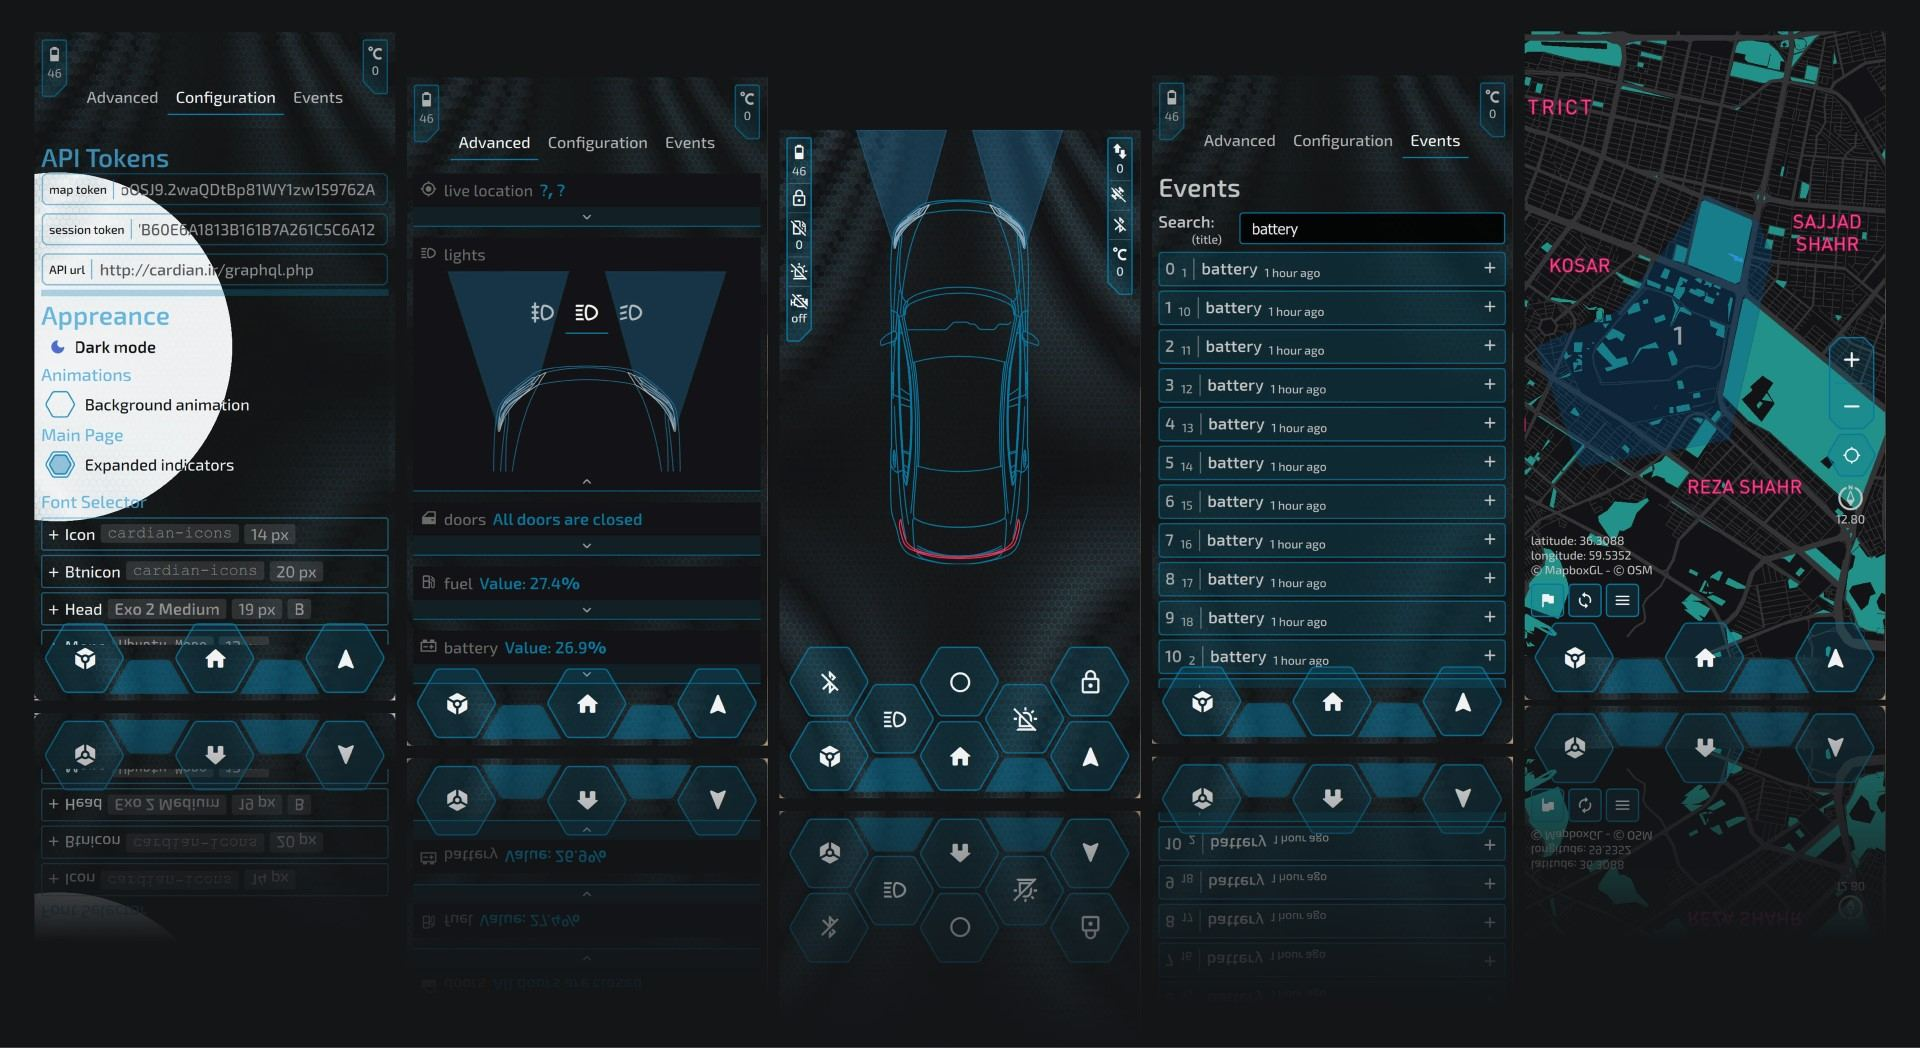
\includegraphics[width=0.7\textwidth]{images/preview-dark.jpeg}
		\caption{حالت تاریک}
		\label{subfig1:fig1:sec2:chap4}
	\end{subfigure}
	\begin{subfigure}[t]{\linewidth}
		\centering
		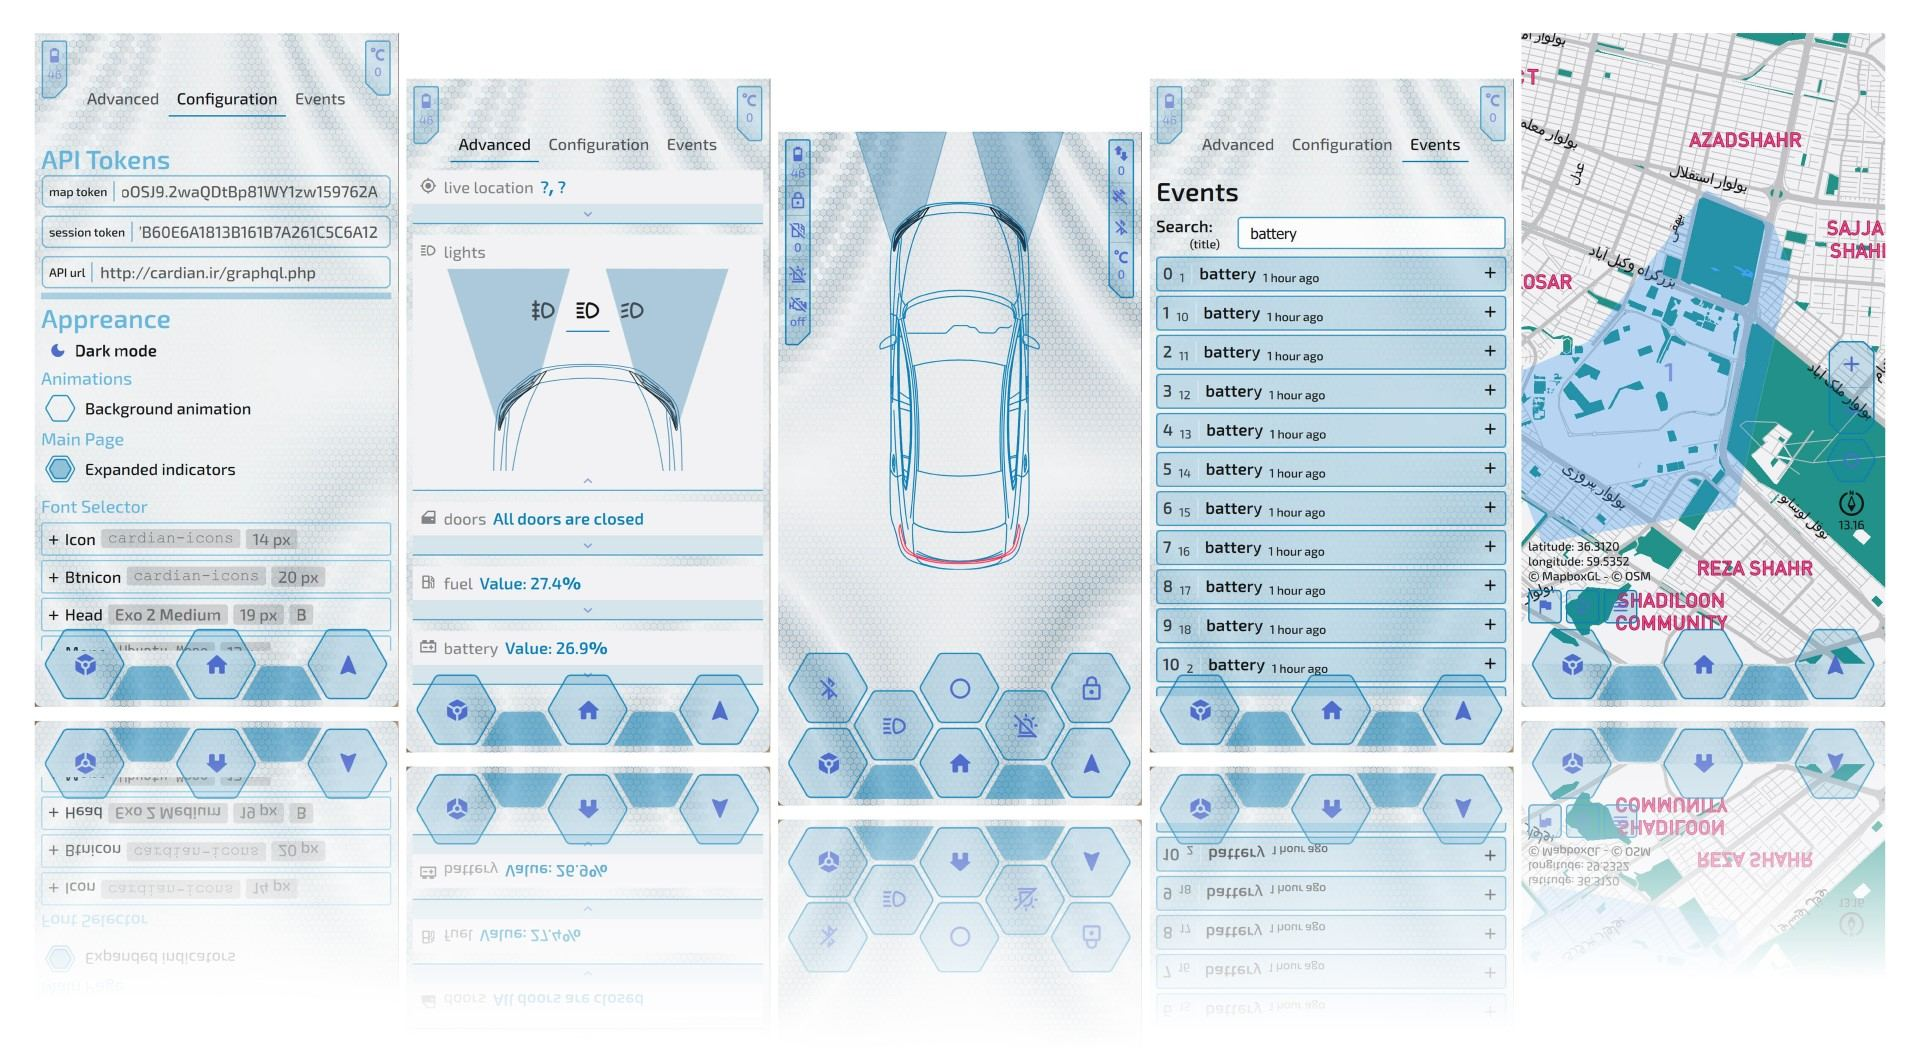
\includegraphics[width=0.7\textwidth]{images/preview-light.jpeg}
		\caption{حالت روشن}
		\label{subfig2:fig1:sec2:chap4}
	\end{subfigure}
	\hspace*{1cm}
	\normalsize
	\label{fig1:sec2:chap4}
	\caption{پیشنمایش‌های برنامهٔ سمت کاربر}
\end{figure}

\section{ساختار برنامهٔ سمت سرور}\label{sec3:chap4}

نقش سرور در پروژه، مطابق با
\hyperref[fig1:sec1:chap4]{دیاگرام معماری پروژه}
 ارتباط بین برنامهٔ سمت کاربر و سخت‌افزار اصلی در خودرو است. که در حال حاضر از زبان پرس‌وجوی \lr{GraphQL} برای ایجاد یک \lr{API} تبادل اطلاعات استفاده شده‌است.

پیاده‌سازی \lr{API} در سمت سرور با استفاده از زبان
\lr{PHP}
انجام شده، علت انتخاب این زبان سادگی و پر استفاده بودن بین مابقی زبان‌ها است. که امکان تهیهٔ
سرویس‌های ارزان‌تر با پشتیبانی پیش فرض از مفسر این زبان تسهیل بخشیده است.


\subsection{زبان برنامه‌نویسی \lr{PHP}}\label{subsec1:sec3:chap4}

یک زبان مفسری همه منظوره و مناسب برای توسعهٔ وب است،‌ این اجازه را به توسعه دهندگان می‌دهد تا بتوانند صفحات پویا و تعاملی وب را طراحی کنند.

\lr{PHP}\LTRfootnote{PHP: Hypertext Preprocessor.}
می‌تواند درون کد‌های \lr{HTML} جاسازی شود،‌با پایگاه‌داده ارتباط برقرار کند.
این زبان متن باز است و شامل گروه‌های بزرگی از برنامه‌نویسان و توسعه‌دهندگان است.

در حال حاضر و در زمان نوشتن این مقاله آخرین نسخهٔ این زبان ۸٫۲ بوده و شامل تغییرات فراوانی نسبت به نسخهٔ پیشین خود یعنی ۷٫۴ داشته است.
\cite{PHPDoc:online}

\subsection{تکنولوژی \lr{GraphQL}}\label{subsec2:sec3:chap4}

\lr{GraphQL}
یک زبان پروس‌وجو برای \lr{API}ها و برای فراهم کردن امکان درخواست\lr{Query}ها است، بدین صورت که اطلاعات کاملی دربارهٔ داده‌های \lr{API} شما به کاربر می‌دهد، و این قدرت را به کاربر می‌دهد تا دقیقاً چیزی رو درخواست کند که نیاز دارد و از هر گونه اطلاعات اضافی صرفه‌نظر شود.

\lr{GraphQL}
با امکان تعریف نوع داده‌ها و تعریف فراهم کننده‌ها در سمت سرور این امکان را فراهم می سازد تا به صورت جزئی برای هر مقدار عملیاتی جدا صورت بگیرد و فقط برای بخش اطلاعاتی که کاربر درخواست کرده پردازش و ارسال اطلاعات صورت بگیرد.

و این امکان را فراهم می‌سازد تا فقط با ارسال یک درخواست تمامی داده‌های مورد نیاز خود را در کمترین حجم داده دریافت کند.

این طریقهٔ ارسال داده کاملاً مناسب با شرایط موجود در ریزپردازنده‌ها و این پروژه است، در حالی که منابع برای پردازش و ارسال چندین درخواست پیاپی موجود نیست و می‌توان با فقط یک درخواست بیشتر داده‌های خواسته شده را بدست آورد.

تکنولوژی \lr{GraphQL} امروزه در مقابل تکنولوژی \lr{SOAP}\footnote{\lr{Simple Object Access Protocol}, یک شیوه‌نامه بر پایهٔ \lr{XML} است.}
 و \lr{REST API} قرار می‌گیرد، و با تسهیل ارسال درخواست و خوانایی بسیار بالا محبوبیت بسیار بالایی در بین توسعه‌دهنده‌ها پیدا کرده‌است.
\cite{GraphQL:online}